As we discussed in the previous section, we decided that we would try to find some available pre-trained models that satisfy our needs. We found 2 models that could use to estimate the 2D human pose from images (AlphaPose and OpenPose). The main difference in these models is the model size, the number of key points that each model predicts per human, and the speed of each model. The accuracy is great for all the models, so it was not a factor to consider. The speed of each model was one of the major factors of each model. Our Hardware could support loading the model on GPU only in the case of the AlphaPose model (which needed 2 GB of VRAM) when the other needed over 3 GB of VRAM. Due to this fact, the difference in speed in AlphaPose was over 30 times faster than the other two models. Another important factor is that AlphaPose had fewer key points, which means that it will have greater accuracy, but poorer quality. At the moment the goal is to create a more stable result, rather than a more attractive one.\\

All the models use the same technique to estimate the 2D pose from the images. They try to estimate some points in the image (x,y) for each joint that they try to find. Therefore, the models predict 18 key points per human that they find in the image, and then with a python library cv2, we connect the dots to create the humanoid. Simpler, having a skeleton with 18 bones, the skeleton from COCO Dataset, the models try to adjust it in every human that they detect in the image. The figures below, demonstrate this procedure.


\begin{figure}[htp]
	\centering
	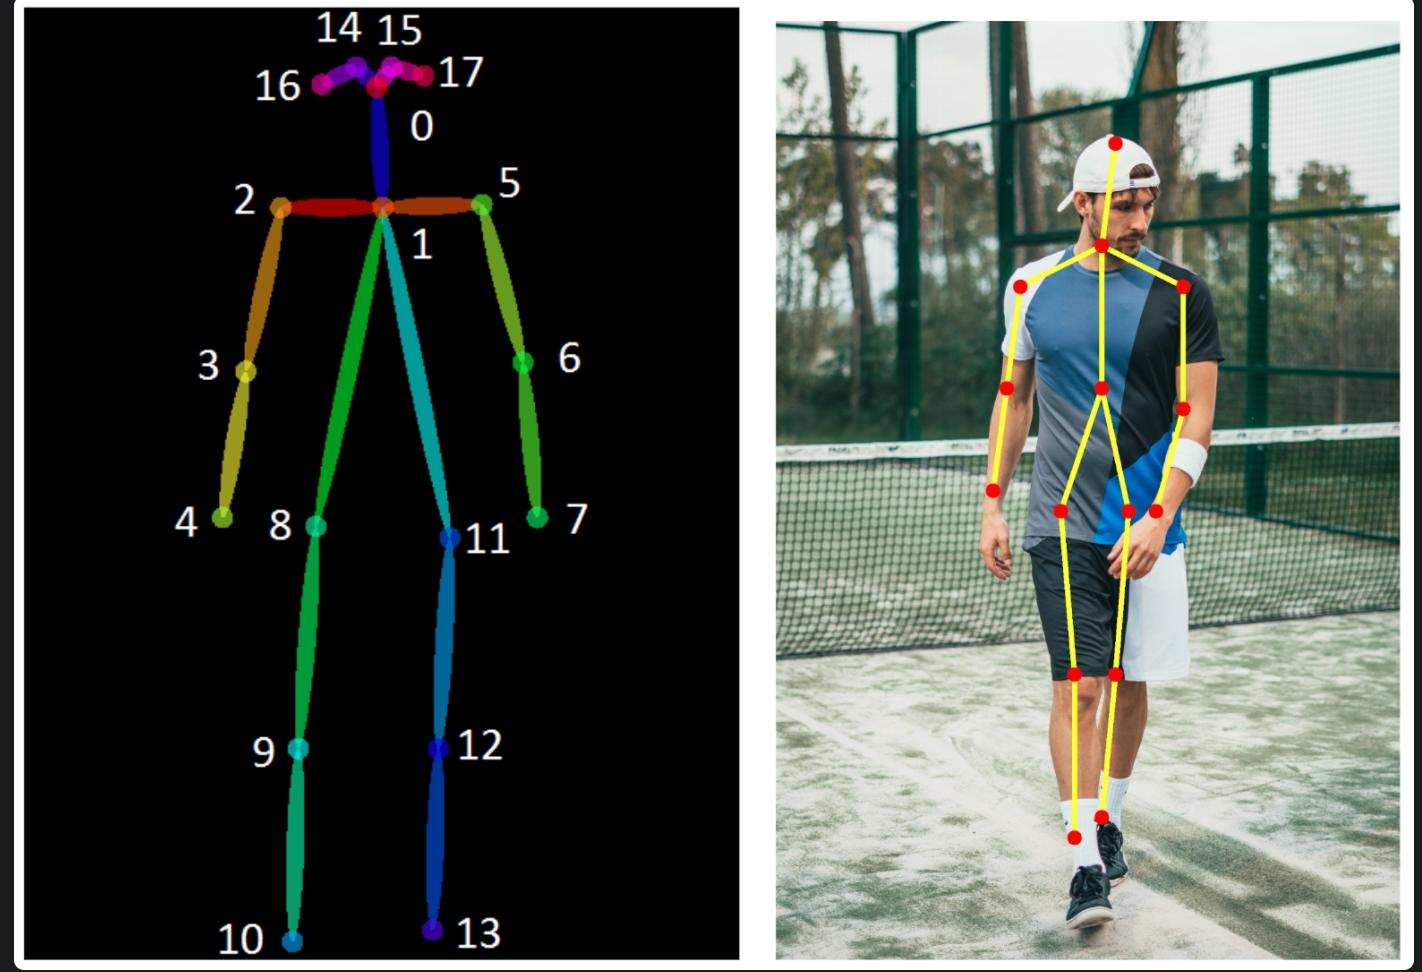
\includegraphics[width=1\textwidth]{figures/Implementation/skeleton.png}
	\captionsetup{labelformat=empty}
    \caption{\href{https://i.stack.imgur.com/sdwNy.jpg}
	{COCO Skeleton that all the models use}}
	\hspace{1em}%
	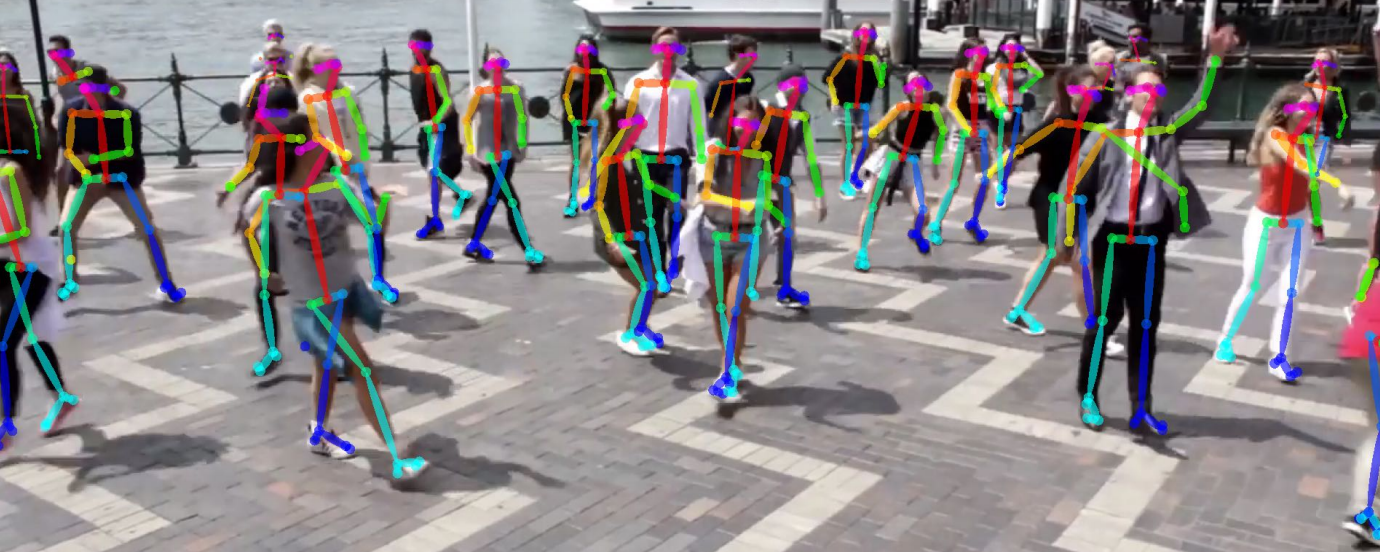
\includegraphics[width=1\textwidth]{figures/Implementation/MultiPerson.png}
	\captionsetup{labelformat=empty}
	\caption{\href{https://github.com/CMU-Perceptual-Computing-Lab/openpose}
	{2D Multi-Human pose Estimation Example}}
\end{figure}

\pagebreak

 \begin{figure}[h]
	\centering
	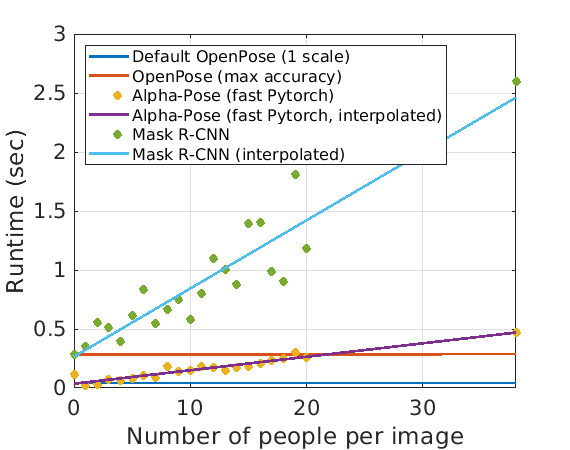
\includegraphics[width=0.75\textwidth]{figures/Implementation/openpose_vs_competition.png}
	\captionsetup{labelformat=empty}
	\caption{\href{https://raw.githubusercontent.com/CMU-Perceptual-Computing-Lab/openpose/master/.github/media/openpose_vs_competition.png}
	{Comparison of each model speed in 2D Multi-Human Pose Estimation}}
\end{figure}

OpenPose model is better and faster when someone wants to detect all the humans that participate in a single image, something that we do not need in this thesis. In the first figure, we show the 2D multi-human pose estimation in an image. In addition, in the second figure, we show the run-time growth for some models with the number of people in the image. Therefore, in our case, for one single person, AlphaPose is the best model in speed and still maintains its max accuracy. Moreover, this OpenPose pre-trained model couldn't be loaded into our GPU, since it wanted more VRAM than we had. Therefore, we would not be able to use this model. In contrast, AlphaPose model could be loaded in our GPU so this played a very important factor when we were choosing the 2D model detector that we were going to use.\\


\subsubsection*{AlphaPose Method}

AlphaPose is a top-down pose estimation algorithm, which chooses Yolo \cite{YOLO-Pose,YOLOv3} as human detector and a single person pose estimator (SPPE) \cite{SPPE} with sequential architecture that detects the human keypoints\\

Yolo model, can classify 80 different objects and segment them inside a box. In our case, the only classification that we need is the human classification, so we can simplify the model in order to get the results faster. Therefore, this model can separate inside a box each human that it can find. Then for each box, we have a single person, and in our case, we will have only one box per frame, since we only accept videos that contain only a single person. \\

In the next step, we have to estimate the human pose of the person inside that box and AlphaPose chose to use the single-person pose estimation. In our case, the pose estimation problem is simplified by only attempting to estimate the pose of a single person, and the person is assumed to dominate the image content. In this model, for a given image, an anchor that is matched against a person stores its entire 2D pose along with a bounding box. For human pose estimation, it boils down to a single class person detection problem with each person having 17 associated keypoints, and each keypoint is again identified with a location and confidence. More specifically, the AlphaPose model can estimate these 17 keypoints per human that can classify inside a box.\\

This SPPE that we discussed about, is a CNN-based method to estimate human poses. The SPPE model is constructed by a simple yet intuitive framework by a series of basic layers such as convolution, pooling, and full connection to learn a mapping from input images to joint coordinates. This network slides over the input image with an overlapped sliding window to detect the presence of joints. More specifically, about the SPPE architecture, we used the summary function from a python machine-learning library (torch) and we display the results in the figure below.

\begin{figure}[h]
	\centering
	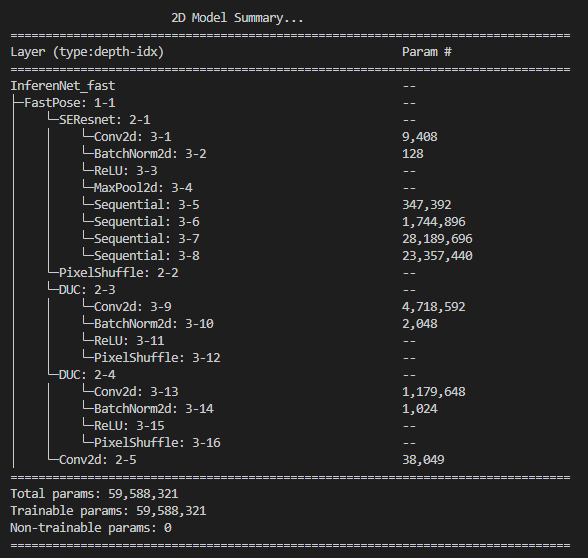
\includegraphics[width=0.7\textwidth]{figures/Implementation/2DModelAr.png}
	\captionsetup{labelformat=empty}
	\caption{2D model summary}
\end{figure}

\pagebreak


\begin{figure}[htp]
    \centering
    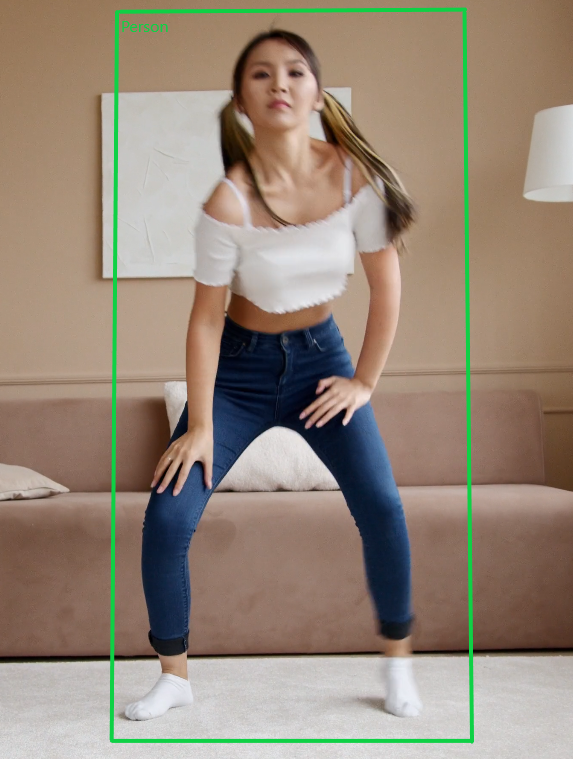
\includegraphics[width=0.4\textwidth]{figures/Implementation/YoloModel.png}%
    \qquad
    
\includegraphics[width=0.4\textwidth]{figures/Implementation/SPPE.png}%
    \qquad
    \captionsetup{labelformat=empty}
    \caption{In the first figure we display the Yolo model Bounding box classification, and in the second the keypoints of the SPPE model}%
\end{figure}


In the above figure, the box estimation is very accurate, but we can see that the keypoints of the model, have a small estimation error on the keypoints that should be symmetrical but are not exactly ( some mm off the right point). We will discuss more about the models estimation errors in the evaluation section.